\chapter{VERIFICATION ENVIRONMENT}
\label{chap:verification.tex}

\section {FUNCTIONAL VERIFICATION}

In SoC design methodology, the first step is to define the specifications. Once the system specifications are completed, design phase starts. The behavioral modeling of the design is done using hardware description languages like VHDL or Verilog HDL and in this stage the design is said to be Register Transfer Level (RTL). Such design could be partitioned to aid reusability, concurrent development and tool effectiveness. In general, reusable components of designs are packaged into components called Intellectual Property (IP). The RTL description of design is verified against functional specifications.  The system level verification is done to verify the RTL description against the intended functionality among other requirements such as timing, power and gate-count. 



Functional verification validates that the design meets the requirements. Test cases are created based on specifications. Various aspects of data and control flow are verified by passing information between external environments, communication with I/O devices,  software interactions etc. [ieee]

 
\section {TEST}

Most SoC verification concentrtes on verifying the processor cores and their interactions with SoC level IPs. At this level of abstraction, verification of interaction between the IPs and functional verification of top level modules are done.  Test conditions are written in x-86 assembly and in some cases written in high level languages like C++. The intension of each test is to verify specific functionality of the design and ensure its validity. The test plans must to be in sync with the specifications of RTL design and are to be updated with new specification changes to ensure that it is efficient enough to deal with all possible corner cases and boundary conditions.

Tests are developed, so that they stimulate the design in a specific manner and compare outcome aganist expected outcome to assert accuracy of design behaviour. Ideally the design should be verified against all possible scenarios that could arise and once it passes all tests, it can be considered as completely verified. In case when a particular test fails, the verification engineer needs to find out the cause of failure with his understanding of design or verification aspect that led to the particular failure. This process of root causing a failure is called as a ``{\it debug}'' in verification. Once root-caused, he then has to suggest appropriate changes to either design, verification or documentation to keep them in unison. 

There are many possible issues that can lead to a test failure. Each test defines conditions for pass and fail. A fail or pass is basically the outcome of a test run. There can be manly different causes for failures, with majority of them being

\begin{description}
	\item[Self check fails]  In a self check failure, the program code running on the simulated processor is able to identify and report a failure. The program tests are written such that they evaluate the results, compare it with desired value and finally report fail or pass. 
	\item[Assertion/Checker fails] Assertion or checker fails are very common kind of failures and occur when a test-bench component reports an unexpected behaviour of either the design or a verification component. In general, most checkers or assertions monitor particular design states during the simulation and report failure whenever monitored value deviates from the expected value. 
\end{description}

In general, a self check fail is caused when program execution deviates from the intended execution flow that was determined for the program under test. Hence the debug of a self check fail would require knowlege of the program under test and its intended execution flow. Without these knowledge, it would be a challenge to debug such fails. This project is aimed to improve debug of such self check fails.

%\subsection {DEVELOP TESTS}
%
%Tests for verifying all the features of the RTL are written in x86 assembly or in high level languages. These test plans are in sync with the specifications of RTL and are to be updated with new specification changes. Test cases should be efficient enough to deal with all possible []: 
%\begin{itemize}
%
%\item Corner cases
%\item Boundary conditions
%\item Design discontinuities
%\item Error conditions
%\item Exception/Interrupt handling
%
%\end {itemize}

\subsection {SELF CHECK FAILURE}

Processor tests are C/assembly program written to assert that the processor under test is indeed functioning as expected under that specific setup. These processor tests are designed such a way that they are capable of deciding if the processor execution results were successful. These tests are normally hand written by the verification engineer rather than randomly generated.  Hence such tests can string together specific stimulus of interest and determine pass or fail status on its own without relying on other verification components. Such tests are called as ``self~tests''.


%\figurename{} 
\begin{figure}[h]
\centering
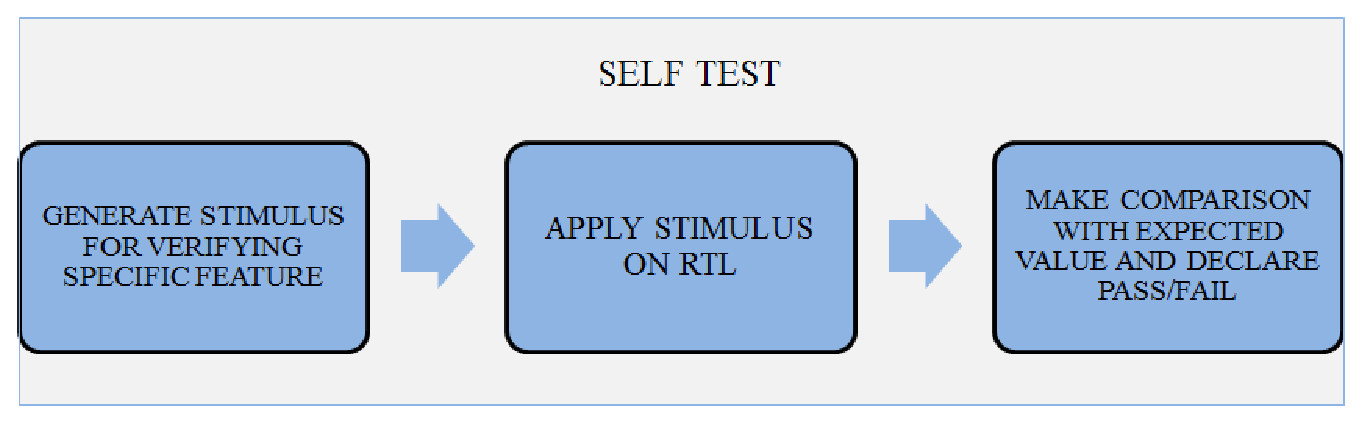
\includegraphics[width=5.5in]{./figures/selftest.ps}
\caption{Self-Test} 
\label{fig:selftest.ps}
\end{figure}

\figurename{\ref{fig:selftest.ps}} details the flow of a self~test. self~tests are a collection of x86 assembly language program. Tests are compiled by a script which calls an assembler followed by a linker. The final output being a linked binary image can be loaded and executed by the RTL model of DUT \nomenclature{DUT}{Design Under Test}. Stimulus is generated by the test and is applied to the DUT. Comparisons are done by the test itself after which pass/fail result is generated.



\section{DEBUGGING A SELF TEST FAILURE}

Self-tests report the occurrence of test case failure. Once this is available, next step is to analyze the reason for failure.  For this, a traceback from the point of failure to the point of error is required. 

A failure message indicates that the result is deviating from the desired value. This desired value can be understood from analysing the asm test code. But to understand at which point during execution the design deviated from the desired course, detailed information regarding execution flow as well as a reference flow which has the ideal values and status are required. In general, a reference flow could be established by the engineer after understanding and interpretting the test in its completeness.
 
To aid execution flow, RTL is simulated along with an instruction level reference simulator. The reference simulator is a software model which imitates the design functionally and executes same instructions in parallel with the RTL. This parallel simulation is also called as co-simulation and produces a log of processor activity.


\subsection {CO-SIMULATION}
The instruction level reference simulator (ILS) \nomenclature{ILS}{Instruction Level Simulator} is an x86/x86-64 compatible model, generally written in software languages such as {\it c++}. It models the processor in great detail including registers, caches and modes of operation. The test provides stimulus to both the RTL and reference models. An interface between RTL and reference model compares the states after each instruction retire and report any mismatch. 

The following section details the features and functions of simulator and interface. 



%\figurename{} 
\begin{figure}[h]
\centering
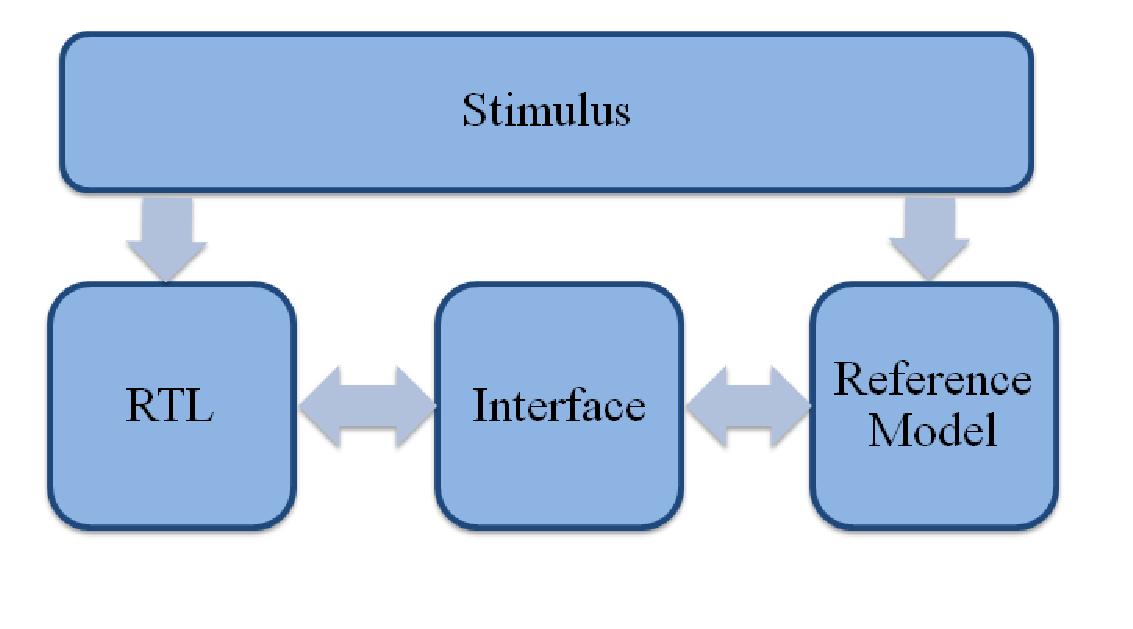
\includegraphics[width=4.5in]{./figures/interface.eps}
\caption{RTL-Reference Model Cosimulation} 
\label{fig:interface.eps}
\end{figure}



%\subsection {COMPARISON WITH REFERENCE MODULE}

%The RTL is simulated along with an instruction level reference simulator. This instruction level simulator is an x86/x86-64 programming model. It mainly models the register states and memory features and act as the ideal reference point to compare with. An interface between RTL and reference model compares the states after each instruction retire and report any mismatch. The following section details the features and functions of simulator and interface.

\subsubsection {INSTRUCTION LEVEL SIMULATOR}
The x86 instruction level simulator starts simulation after initializing the contents of its memory with linked binary image of the test. The ILS emulates the fetch/decode/execute algorithm of a scalar processor, producing an output log known as processor execution log. Each log entry describes the instruction, its results and any side effects it had on the processor state. The simulator models debug features, exceptions and interrupts as well as processor specific features. Supported processor states include x86 general purpose registers, flag registers, control registers, media registers, model specific registers as well as memory and I/O spaces. The simulator runs multi-threaded code to simulate multi-processor and multi-core processor systems. 
The simulator runs in step with the RTL. Whenever an instruction or exception is retired in RTL that thread within the simulator is stepped-up and the processor states in the RTL and the simulator are compared. Difference detected in processor states are considered as a mismatch; difference in memory locations are also considered as mismatches and upon any mismatch, the co-simulation is terminated. At the end of the simulation when all threads stop executing, the memory states of RTL and the simulator are compared and any discrepancies are reported as memory mismatches.

\subsubsection {INTERFACE}
The interface between RTL and reference model keeps the ILS in step with RTL signal. It steps the ILS when an instruction in RTL simualtion has retired and then compares the results of execution between RTL and ILs. If the reference model is unable to model anything that is present in the RTL, the interface also re-synchronizes the ILS with the state obtained after execution of the RTL instruction.
Main functions of this interface includes
\begin{description}
	\item[Initialization] Initialize memory model, attach RTL signal and initialize some specific RTL signals.
	\item[Increment] Based on number of instruction retired per cycle, the interface informs ILS how many instructions to step.
	\item[Interrupt Handling] Interface informs ILS about pending interrupts
	\item[Comparing] Compares RTL and reference model registers; integer, FP, control and status word. Also reports any mismatches.
	\item[Interfacing with the memory model] Tell memory model what operations are seen by the RTL. 
\end{description}

\label{verif:exelog}
During the course of simulation, the ILS generates log files holding processor's program execution details. These are called ``\emph {processor execution log}''s. These log files will contain cycle by cycle information regarding register states, memory values, flags, threads etc. Basically all the comparison and debugging will require these information.

Once a failure is reported, simulation terminates and it would be required to be debugged. For root-causing the failure, verification engineer needs to trace through this processor execution log. Mismatches with reference model values provide information regarding the cause of failure.

Tracing through the log files is done manually. Data obtained from instruction simulation log and the assembled test files needs to be analyzed and co-related for debugging the failure. This is a very tedious effort consuming a lot of verification time. This is because of two main reasons:

\begin{enumerate}
	\item Relevant/required information is buried under a wealth of information
	\item Co-related information is spread across in different files
\end{enumerate}

As the design itself is very complex, these reasons makes manual tracing too time consuming. This will stretch the verification time and ultimately time-to-market.   


